% Working draft targeting CVPR 2027, updated 2026-10-23.
% Uses the unmodified official CVPR 2026 author-kit style provisionally.
\documentclass[10pt,twocolumn,letterpaper]{article}
\usepackage[T1]{fontenc}
\usepackage[review]{cvpr}
\usepackage{tikz}
\usetikzlibrary{arrows.meta,positioning}
\definecolor{cvprblue}{rgb}{0.21,0.49,0.74}
\usepackage[pagebackref,breaklinks,colorlinks,allcolors=cvprblue]{hyperref}
\def\paperID{*****}
\def\confName{CVPR}
\def\confYear{2027}
\newcommand{\method}{EPHS\xspace}
\newcommand{\pending}{\textcolor{gray}{--}}
\newcommand{\draftnote}[1]{\par\noindent{\small\color{cvprblue}\textbf{Draft status.} #1}\par}
\title{Evidence-Preserving Head Steering\\for Context-Robust Object Grounding}
\author{Anonymous Authors}
\begin{document}
\maketitle
\begin{abstract}
Object grounding requires a vision--language model to distinguish evidence of
an object's presence from contextual cues that merely make the object likely.
Reducing hallucinations by making a model more reluctant to answer positively
can obscure this distinction and increase omissions of genuinely visible
objects. We study whether a small intervention in attention-head outputs can
improve this tradeoff. We propose Evidence-Preserving Head Steering
(\method), which separates offline causal localization from supervised
intervention fitting. Localization contrasts activation-patching effects on
target-occluded images with effects on matched background controls. The
selected heads receive bounded scalar gains, fitted with balanced
object-existence supervision and a distribution-preservation objective while
the pretrained backbone remains frozen. Inference requires only the input
image and question, without donor activations or object annotations. We
specify an evaluation protocol that separates sensitivity to object presence
from sensitivity to surrounding context, alongside natural-image
hallucination, object recall, and capability measurements. The central
hypothesis is that control-adjusted head selection improves object grounding
beyond response-threshold calibration and equally sized arbitrary
interventions. This draft presents the implemented method and the protocol
for testing that hypothesis; empirical performance remains to be established.
\end{abstract}

\draftnote{Research draft, October 23, 2026. Benchmark experiments are pending.
Dashed table entries are unmeasured, not zero. The official 2026 author kit is
used provisionally for a 2027 submission; the 2027 format must be rechecked.}
\section{Introduction}
\label{sec:intro}

An image of a tennis racket can make a ball plausible without making it
visible. A grounded vision--language model (VLM) should distinguish these
cases: it should recognize a clearly visible ball even without familiar
surrounding objects, and reject its presence when only those contextual cues
remain. This distinction matters for descriptions and visual question
answering, where a plausible but unsupported object can change the meaning
of a response. Object hallucination has been documented in image captioning
and modern VLMs~\cite{chair,pope}. Counterfactual removal and contextual
interventions further expose failures that aggregate accuracy can
conceal~\cite{removedobjects,causalhalbench}.

We focus on a narrow requirement: \emph{object-presence judgments should
respond to changes in the target object while remaining correct under
changes to surrounding context that preserve its presence}. These are
complementary requirements. A model that answers \emph{no} more often may
reduce false positives while missing more real objects. A model that repeats
the same answer across edited images may appear context-invariant while
being consistently wrong. Evaluation must therefore measure both sides of
the decision, and correctness across related images, rather than rewarding
invariance or lower hallucination in isolation.

Recent steering approaches offer alternatives to updating all model
parameters. VTI intervenes in visual and textual representations, GrAInS uses
gradient-based attribution, REVIS aims to restore suppressed visual
information, and RUDDER reinforces evidence extracted from residual
updates~\cite{vti,grains,revis,rudder}. These approaches motivate studying
where an intervention should act. However, their existence also raises the
standard for a new method: stronger visual features or sparse intervention
alone is not a sufficient methodological contribution.
HONES already connects causal head localization to sparse neuron
scaling~\cite{hones}, and recent work explicitly investigates visual-context
sensitivity and spurious associations~\cite{seeingknowing,purge}.

Our hypothesis concerns the \emph{selection criterion} and the
\emph{preservation-constrained intervention}. We ask whether heads selected
for a target-specific information-transfer effect provide more useful
intervention sites than equally many randomly chosen or high-magnitude
heads. Evidence-Preserving Head Steering (\method) first substitutes clean
head activations into target-occluded inputs and into matched background
controls. It ranks heads by the former effect after penalizing the latter,
then learns small head-wise gains on separate, balanced examples. A
preservation term discourages changes to the base model's next-token
distribution on examples it originally answers correctly.

Crucially, these steps have different meanings. Restoring a clean activation
to an object-occluded image is a diagnostic of information transfer; it can
restore an answer that is incorrect for the edited image. It does not show
that amplifying the same head improves deployment. Likewise, a matched
background occlusion controls some edit-related effects but does not isolate
semantic context. We therefore evaluate the learned gains using single
images, without donors, and reserve semantic-context interventions as a
separate test of the motivating hypothesis.

This work is organized around three proposed contributions: a
control-adjusted head-localization criterion; bounded gain fitting with
balanced supervision and preservation of correct base-model distributions;
and a comparison protocol that tests whether any improvement exceeds answer
bias calibration, arbitrary head interventions, and existing steering
methods. The first two have a CPU-tested implementation. Their empirical
benefit, the semantic-context protocol, and the adequacy of the comparison
to close prior work remain to be established. We do not claim a new
hallucination phenomenon or a new benchmark.

\begin{table}[t]
\centering
\small
\begin{tabular}{lll}
\toprule
Target object & Associated context & Correct answer \\
\midrule
Present & Present & Yes \\
Absent & Present & No \\
Present & Absent & Yes \\
Absent & Absent & No \\
\bottomrule
\end{tabular}
\caption{The intended diagnostic distinguishes target evidence from
associated context. Each question asks about the same target category.
These are experimental conditions, not observed model results. Correctness
must be assessed in every condition; constant answers are insufficient.}
\label{tab:conditions}
\end{table}

\section{Related Work}
\label{sec:related}

\paragraph{Object hallucination and contextual shortcuts.}
CHAIR measures unsupported object mentions in captions, while POPE evaluates
object existence with controlled negative-object sampling~\cite{chair,pope}.
Their complementary response formats make it possible to inspect both
generated descriptions and binary decisions. They do not, by themselves,
identify the computational origin of a failure. He
et al.~\cite{removedobjects} evaluate hallucinations after object removal and
propose object-focused preference optimization. Causal-HalBench formalizes
co-occurrence-induced spurious correlations and evaluates counterfactual
images~\cite{causalhalbench}. We build on these problem formulations; target
removal and contextual evaluation are not introduced here.

\paragraph{Activation steering in VLMs.}
VTI modifies visual and textual latent representations to reduce
hallucination~\cite{vti}. GrAInS derives steering directions from
gradient-based attribution of preferred versus dispreferred
outputs~\cite{grains}. REVIS constructs a purified visual direction and
calibrates sparse intervention, while RUDDER obtains an evidence direction
from prefill residual updates and applies adaptive
reinforcement~\cite{revis,rudder}. \method instead fits scalar gains on
selected, pre-projection attention-head outputs. This architectural
difference is an experimental choice, not evidence of superiority. It
requires comparison at matched preprocessing, decoding, calibration budget,
and object recall.

\paragraph{Localization and targeted parameter changes.}
HONES localizes task-relevant heads, attributes their downstream effects to
FFN neurons, and learns sparse neuron scaling~\cite{hones}. It is especially
close to our localization-then-scaling design. Seeing or
Knowing?~\cite{seeingknowing} examines visual-context sensitivity and connects
internal intervention analysis with steering. PURGE studies partition-aware
unlearning of spurious associations while preserving object
reasoning~\cite{purge}. Consequently, neither causal localization, selective
scaling, nor evidence--context separation is a first-of-its-kind claim for
\method. Its narrower candidate contribution is whether the
target-versus-control patch score selects better sites for bounded
head-output gains under information-preserving evaluation.

\paragraph{Scope of the comparison.}
Frozen-backbone steering and unlearning or preference optimization incur
different training costs and use different supervision. We report those
differences rather than treating all methods as equally resource-free.
Our four existing steering implementations are local adaptations, not
verified reproductions of published scores. Comparisons to HONES, the
visual-context steering method, and PURGE require additional implementation
or integration before a scientific claim can be made.

\section{Evidence-Preserving Head Steering}
\label{sec:method}

\begin{figure*}[t]
\centering
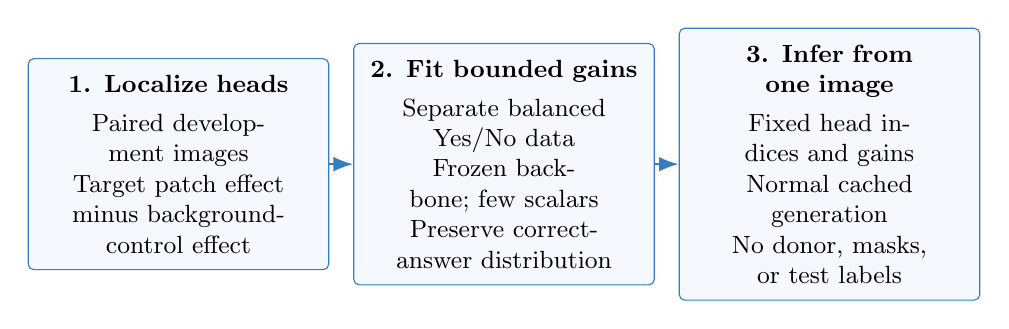
\begin{tikzpicture}[
  box/.style={draw=cvprblue,rounded corners=2pt,fill=cvprblue!5,
    align=center,text width=0.28\textwidth,minimum height=2.1cm,
    inner sep=6pt,font=\small},
  link/.style={-{Latex[length=2.5mm]},thick,color=cvprblue}]
\node[box] (discover) {
  \textbf{1. Localize heads}\\[3pt]
  Paired development images\\
  Target patch effect\\
  minus background-control effect};
\node[box,right=0.025\textwidth of discover] (fit) {
  \textbf{2. Fit bounded gains}\\[3pt]
  Separate balanced Yes/No data\\
  Frozen backbone; few scalars\\
  Preserve correct-answer distribution};
\node[box,right=0.025\textwidth of fit] (infer) {
  \textbf{3. Infer from one image}\\[3pt]
  Fixed head indices and gains\\
  Normal cached generation\\
  No donor, masks, or test labels};
\draw[link] (discover) -- (fit);
\draw[link] (fit) -- (infer);
\end{tikzpicture}
\caption{The implemented \method pipeline. Localization and fitting use
disjoint development images. Patching is an offline oracle diagnostic,
whereas deployment applies learned scalar gains to a single input.
Semantic-context robustness is an evaluation hypothesis, not a property
guaranteed by the localization score.}
\label{fig:pipeline}
\end{figure*}

\subsection{Task and intervention site}
Given an image $x$ and a question $q$ about the existence of a target
category, let $m(x,q)=z_{\mathrm{Yes}}-z_{\mathrm{No}}$ denote the base model's
first-answer-token logit margin. The configured affirmative and negative
strings must each correspond to one distinct token. This forced-choice
quantity is used for localization and fitting; it is distinct from the
accuracy of freely generated answers.

At decoder layer $\ell$, let $u_{\ell,h,t}$ be the output of query head $h$
at position $t$, before the attention output projection mixes heads. The
implementation hooks the concatenated input of that projection and selects
the corresponding head slice. For grouped-query attention, the split uses
the number of query heads, not the number of key/value heads. We do not
modify attention probabilities or claim that the selected head is an
independent semantic feature.

\subsection{Control-adjusted causal localization}
\label{sec:localize}
Each discovery record provides a clean image $x$, a target-occluded image
$x^{-}$, a background-control image $x^{c}$, and the same question $q$.
The current COCO builder unions the segmentation masks of all annotated
instances of the target category and fills the union with gray. A control
is created by translating the same mask shape onto background that excludes
annotated objects. Records without a valid matched control are unsuitable
for this analysis. Annotation incompleteness and the limits of occlusion
as an intervention must be assessed separately.

We retain positive records for which the base model's clean forced-choice
answer is correct, $m(x,q)>0$, and target occlusion decreases the margin by
$d=m(x,q)-m(x^{-},q)>\epsilon$. For each candidate head, we replace its final
prompt-position activation in $x^{-}$ with the corresponding activation
from $x$, and repeat this operation for $x^{c}$. Writing the resulting
margin changes as $r_{\ell,h}$ and $c_{\ell,h}$, respectively, the score is
\begin{equation}
 s_{\ell,h}(x,q)=
 \frac{r_{\ell,h}-\lambda_c |c_{\ell,h}|}
      {\max(d,\eta)}.
 \label{eq:score}
\end{equation}
The denominator floor $\eta$ avoids treating tiny margin changes as strong
evidence. The control penalty discourages heads whose clean substitution
also strongly changes the matched control input. Scores are averaged over
questions from each original image, then aggregated by their median across
image groups. The top $K$ heads form the selected set $\mathcal{S}$.

The current selector always returns the top $K$ candidates; it does not
require positive scores. Therefore, selection alone must not be interpreted
as proof that useful heads were discovered. We inspect score signs,
between-image variability, and stability across discovery samples before
interpreting a selected set. Random-head and clean-activation-RMS selectors
use the same candidate pool for controlled comparisons.

\paragraph{What this intervention establishes.}
A clean donor carries information about an object that the occluded input
does not contain. Successful patching can consequently increase an
\emph{incorrect} positive answer on the occluded image. Its role is to
identify a route by which the clean input affects the answer, not to count
a corrected prediction. The background control only adjusts for some
occlusion-related effects. It neither identifies a unique causal pathway
nor proves invariance to semantic context. The usefulness of
Eq.~\eqref{eq:score} is tested by subsequent single-input intervention,
not assumed.

\subsection{Bounded gains with distribution preservation}
\label{sec:fit}
On a separate fitting split, we freeze the pretrained model and optimize
one scalar $a_{\ell,h}$ per selected head. Its bounded gain is
$\delta_{\ell,h}=\rho\tanh(a_{\ell,h})$, initialized at zero, and its output
is transformed as
\begin{equation}
 \widetilde u_{\ell,h,t}=
 \begin{cases}
 (1+\delta_{\ell,h})u_{\ell,h,t},
       &(\ell,h)\in\mathcal{S},\\
 u_{\ell,h,t},&\text{otherwise}.
 \end{cases}
 \label{eq:gain}
\end{equation}
With $\rho=0.25$, the multiplier remains between $0.75$ and $1.25$.
The intervention cannot reverse or eliminate a head. Both amplification
and attenuation are learned; a high patch score does not prescribe their
sign.

Let $y\in\{-1,+1\}$ be the object-existence label, $m_\delta$ the steered
margin, and $p_0$ and $p_\delta$ the full-vocabulary next-token distributions
at the final prompt position. The fitting objective is
\begin{equation}
\begin{split}
\mathcal{L}={}&
 \mathbb{E}_{\mathrm{bal}}\left[
 \operatorname{softplus}(-y m_\delta)
 +\lambda_{\mathrm{KL}} I_{\mathrm{keep}}
   D_{\mathrm{KL}}(p_0\Vert p_\delta)\right]\\
 &+\frac{\lambda_2}{K}
   \sum_{(\ell,h)\in\mathcal{S}}\delta_{\ell,h}^{\,2}.
\end{split}
\label{eq:loss}
\end{equation}
Balanced sampling pairs positive and negative examples, cycling the smaller
class to give both labels equal exposure. $I_{\mathrm{keep}}$ is one only
when the base forced-choice answer is correct and the record is eligible
for preservation. Eligibility is fixed by the data protocol, not chosen
after inspecting intervention outcomes.

The KL term regularizes a single next-token distribution; it does not
guarantee preservation of a generated caption or general reasoning.
Those properties require held-out evaluation. Although the backbone is
frozen, fitting uses supervision and backpropagation, so \method is not
training-free.

\subsection{Deployment and computational requirements}
The default intervention affects only the final prefill token and the
current token at each cached decoding step. Earlier prompt positions are
unchanged. An all-prefill-position variant is a separate ablation, and its
setting must match between fitting and deployment. The deployed artifact
contains the head indices, gains, and intervention-position setting.

Inference uses the original image and question, without edited images,
clean donors, ground-truth labels, or a per-example backward pass. It uses
one normal generation path, but hooks and head-wise operations still incur
overhead; no latency benefit is assumed. Localization is more expensive:
each discovery record requires three base forwards and each retained
record requires two additional forwards per candidate head. Fitting also
requires backward computation through the frozen network. We report these
offline costs separately from inference cost.

\subsection{Semantic-context robustness as a testable hypothesis}
The implemented method does not optimize an explicit semantic-context
invariance loss. Its proposed connection to context robustness is that
target-selective localization may expose intervention sites that help
preserve useful visual evidence. This connection is falsifiable. If gains
selected by Eq.~\eqref{eq:score} fail on semantic-context edits, or perform
no better than gains on arbitrary heads, the motivating mechanism is
unsupported even if a standard hallucination score improves.

\section{Experimental Protocol}
\label{sec:experiments}
\draftnote{This section specifies intended experiments. Dataset sizes and
hyperparameters below are pilot configurations, not completed runs or
validated choices.}

\subsection{Models and disjoint development splits}
The primary model is Qwen2.5-VL-7B-Instruct~\cite{qwen25vl}. We will test
transfer to Qwen3-VL-8B-Instruct~\cite{qwen3vl} and Gemma 4 E4B-it~\cite{gemma4}.
The two Qwen models test transfer across generations, while Gemma 4 tests
a different model family. E4B has 4.5B effective parameters and 8B total
including embeddings; absolute scores across models are not capacity-matched.
We will pin exact model and
processor revisions and use the same image preprocessing, prompts, decoding
settings, and evaluation examples for every method on a given model.
Current configurations use batch size one, BF16, eager attention, a
448-square input preprocessing step, and greedy cached generation.
The model-specific processor may apply further resizing; the effective
image and token dimensions must be recorded.

COCO train images~\cite{coco} supply disjoint discovery, fitting, and
hyperparameter-tuning groups. An initial development allocation is 200
original images per split, with at most 100 discovery records processed
by the starting configuration. All questions and edited variants of an
original image remain in the same group. COCO validation images and
external evaluations are checked for original-image overlap rather than
assumed independent because benchmark names differ.

Initial \method settings are $K=8$, $\lambda_c=1$, $\eta=1$, and
$\epsilon=0.05$. Candidate decoder layers are $\{8,12,16,20,24\}$ for the
two Qwen models and $\{5,11,23,35,41\}$ for Gemma 4 E4B; the latter five
are full-attention layers. All query heads in these layers are considered.
Gains use Adam for two balanced epochs
with learning rate $0.03$, $\rho=0.25$, $\lambda_{\mathrm{KL}}=1$, and
$\lambda_2=0.01$. These settings are starting points. Any tuning will use
development data and a declared budget before final evaluation.

\subsection{Evidence and context diagnostics}
The primary diagnostic follows Table~\ref{tab:conditions}. Each original
image group should support target-present and target-absent conditions,
crossed with the presence or absence of an associated contextual cue.
Target identity, visibility, and position should be preserved when changing
context; context should be preserved as far as possible when removing the
target. Image edits require quality checks for residual objects, boundary
artifacts, unintended semantic changes, and ambiguous labels.

This semantic-context diagnostic is a \emph{planned addition}; the current
gray-occlusion builder does not supply it. We will also evaluate the
unchanged Causal-HalBench test material and its official metrics rather
than repurpose that benchmark as method-selection data~\cite{causalhalbench}.
Native benchmark fields and metric names will be preserved.

We will report accuracy for each condition and the fraction of complete
four-condition groups for which every answer is correct. For controlled
target changes, both answers must be correct; merely flipping the answer
does not count as success. For context-only changes, both answers must
again be correct; constant wrong answers receive no credit.

\paragraph{Separating discrimination from response bias.}
For forced-choice answers, we will compare false-positive rates at
development-calibrated operating points with similar true-positive rates,
and report the achieved test rates rather than assume exact matching.
Thresholds are chosen only on the tuning split. ROC curves provide a
complementary threshold-sweep diagnostic. A base-model margin-offset
baseline changes the Yes/No threshold without changing representations.
This control is essential: a global score shift must not be mistaken for
improved evidence discrimination.

\subsection{Natural images, information retention, and capability}
POPE random, popular, and adversarial subsets provide natural-image
object-existence evaluation~\cite{pope}. We report accuracy, precision,
recall, F1, affirmative-answer rate, and invalid-response rate. Generated
answers use the same parser; malformed or noncommittal answers are not
silently discarded.

On an intended 2,000-image COCO validation subset, we will measure
CHAIR$_s$ and CHAIR$_i$ alongside correct object recall, distinct correct
object mentions, and actual caption length~\cite{chair,coco}.
Generation limits are matched, and multiple steering strengths are used to
inspect the hallucination--recall relationship. The CHAIR object taxonomy
does not establish correctness of every attribute or relation.
MME supplies an additional capability-retention check~\cite{mme}.
MMHal-Bench supplies 96 free-response hallucination questions~\cite{mmhal}.
We will use its official response format and one fixed judge version and
scoring prompt for all methods on a model. Judge outputs and response
lengths will be retained; its score is not treated as a Yes/No accuracy.

\subsection{Baselines and implementation parity}
The comparison includes the unmodified model, threshold calibration,
VTI, GrAInS, REVIS, and RUDDER. HONES and the steering method studied in
Seeing or Knowing? are close mechanistic comparators; PURGE and
object-focused preference optimization provide relevant training-based
comparisons where computational and data budgets permit.

The current four steering ports use a common runtime but contain material
adaptations. GrAInS attributes fused decoder-input embeddings from a zero
baseline; VTI uses a fixed visual grid; REVIS uses a fixed neutral-response
choice; and RUDDER exposes an explicit first-token intervention choice.
Common COCO Yes/No preference pairs also differ from original caption
preference data. Therefore, the present ports must be labeled
\emph{adapted}, and checked against author implementations on shared small
inputs before results are presented as reproductions.

Every method receives a declared development and tuning budget. We account
for \method's segmentation masks, paired edits, labels, and discovery
computation, not only the number of fitted parameters. Published scores
from different experimental settings will not be inserted into the same
comparison table.

\subsection{Ablations and uncertainty}
Required ablations replace causal selection with random or activation-RMS
selection while keeping the same $K$, candidate pool, fitting data, and
optimization budget. Further tests remove the control penalty or the KL
term, vary $K$ and the gain bound, and compare last-token with all-prefill
intervention. A residual-scaling control tests whether a generic magnitude
change explains the effect.

We will repeat discovery and fitting with at least three specified seeds
and report all runs. Paired confidence intervals resample original image
groups, keeping correlated questions and variants together; seed
variability is reported separately. Inference timing uses synchronized GPU
measurements after warm-up and is accompanied by peak memory, output
length, and the actual device configuration.

\section{Results and Analysis Plan}
\label{sec:results}
\draftnote{No pretrained checkpoint from the three-model protocol has been
evaluated for this study.
The tables below are reporting layouts and contain no measured model
performance.}

\begin{table*}[t]
\centering
\small
\setlength{\tabcolsep}{4pt}
\begin{tabular}{lccccccc}
\toprule
 & \multicolumn{4}{c}{Condition accuracy $\uparrow$}
 & \multicolumn{3}{c}{Grounding diagnostic}\\
\cmidrule(lr){2-5}\cmidrule(lr){6-8}
Method & $O^+C^+$ & $O^-C^+$ & $O^+C^-$ & $O^-C^-$
 & All four $\uparrow$ & FPR $\downarrow$
 & Achieved TPR $\uparrow$\\
\midrule
Base & \pending & \pending & \pending & \pending & \pending & \pending & \pending\\
Base + threshold & \pending & \pending & \pending & \pending & \pending & \pending & \pending\\
VTI (adapted) & \pending & \pending & \pending & \pending & \pending & \pending & \pending\\
GrAInS (adapted) & \pending & \pending & \pending & \pending & \pending & \pending & \pending\\
REVIS (adapted) & \pending & \pending & \pending & \pending & \pending & \pending & \pending\\
RUDDER (adapted) & \pending & \pending & \pending & \pending & \pending & \pending & \pending\\
HONES (pending) & \pending & \pending & \pending & \pending & \pending & \pending & \pending\\
Random heads + gain fit & \pending & \pending & \pending & \pending & \pending & \pending & \pending\\
\method & \pending & \pending & \pending & \pending & \pending & \pending & \pending\\
\bottomrule
\end{tabular}
\caption{Planned forced-choice comparison on Qwen2.5-VL-7B. $O$ denotes target
presence and $C$ associated-context presence. All four requires every
condition in a complete original-image group to be correct. Condition and
group accuracy use the zero margin threshold, except for the calibrated
Base + threshold control. FPR and achieved TPR use separately
development-selected operating points for every method. Generated-answer
and caption metrics are reported separately. No entries have been measured.
Additional close comparators in Sec.~\ref{sec:related} remain necessary
before finalizing the table.}
\label{tab:main}
\end{table*}

\begin{table*}[t]
\centering
\small
\setlength{\tabcolsep}{4pt}
\begin{tabular}{llccccc}
\toprule
Model & Method & POPE F1 $\uparrow$ & CHAIR$_i$ $\downarrow$
 & Obj. recall $\uparrow$ & MME $\uparrow$ & MMHal $\uparrow$\\
\midrule
Qwen2.5-VL-7B & Base & \pending & \pending & \pending & \pending & \pending\\
 & Best adapted baseline & \pending & \pending & \pending & \pending & \pending\\
 & \method & \pending & \pending & \pending & \pending & \pending\\
Qwen3-VL-8B & Base & \pending & \pending & \pending & \pending & \pending\\
 & Best adapted baseline & \pending & \pending & \pending & \pending & \pending\\
 & \method & \pending & \pending & \pending & \pending & \pending\\
Gemma 4 E4B & Base & \pending & \pending & \pending & \pending & \pending\\
 & Best adapted baseline & \pending & \pending & \pending & \pending & \pending\\
 & \method & \pending & \pending & \pending & \pending & \pending\\
\bottomrule
\end{tabular}
\caption{Planned three-model transfer comparison. The strongest adapted
baseline is selected separately on development data for each model; the
full method-wise results and output lengths will also be reported. Model
capacities differ, so conclusions concern within-model changes from Base.
All entries are unmeasured.}
\label{tab:transfer}
\end{table*}

\subsection{Implementation verification}
The implementation has passed 74 local CPU correctness tests and static
code checks. Tests include tensor interventions, gradient flow to bounded
gains, restoration of hooks and base weights, data-group separation, and
evaluation adapters. Small randomly initialized instances of the actual
Qwen2.5-VL, Qwen3-VL, Gemma 4, and LLaVA architecture classes exercise image inputs,
grouped-query head slicing, and cached generation. These tests establish
software behavior under their test conditions. They do not reproduce
published baseline scores, establish usefulness of the selected heads, or
predict pretrained-model performance.

\subsection{Does the intervention improve grounding?}
Table~\ref{tab:main} is designed to expose whether fewer false positives
come at the expense of real-object recognition. The intended supporting
pattern is improved performance in the target-absent, associated-context
condition without deterioration when a target is present without its usual
context. A stronger claim requires improvement in complete-group
correctness and in discrimination beyond the base threshold control.
If only the operating point changes, we will report that narrower outcome.

\subsection{Does causal selection matter?}
The crucial comparison holds gain fitting fixed and changes only head
selection. We will inspect whether control-adjusted selection outperforms
random and magnitude-based choices across discovery samples. We will also
compare localization scores with held-out intervention effects, rather
than infer the latter from patch recovery. Unstable selected sets, uniformly
nonpositive scores, or no advantage over random heads would weaken the
proposed mechanism.

\begin{table}[t]
\centering
\small
\setlength{\tabcolsep}{2.5pt}
\begin{tabular}{lcccc}
\toprule
Variant & CHAIR$_i$ $\downarrow$ & Rec.\ $\uparrow$
 & Length & All four $\uparrow$\\
\midrule
Base & \pending & \pending & \pending & \pending\\
Best baseline & \pending & \pending & \pending & \pending\\
\method & \pending & \pending & \pending & \pending\\
No KL & \pending & \pending & \pending & \pending\\
No control penalty & \pending & \pending & \pending & \pending\\
Random heads & \pending & \pending & \pending & \pending\\
\bottomrule
\end{tabular}
\caption{Planned preservation and selection ablations. Rec.\ denotes object
recall. The strongest steering baseline is selected using development
data. Actual caption length is reported because an identical maximum token
budget does not ensure equally informative outputs. All values are pending.}
\label{tab:ablation}
\end{table}

\subsection{Does information preservation transfer?}
Table~\ref{tab:ablation} tests whether first-token regularization transfers
to descriptions. Lower CHAIR with substantially shorter captions or lower
object recall would not demonstrate the intended benefit. We will inspect
hallucination--recall curves and MME changes across all three models, and
report mixed or negative outcomes explicitly. Semantic-context, natural-image,
and capability results should support compatible conclusions before
describing \method as context-robust.

\section{Limitations}
\label{sec:limitations}

The most immediate limitation is the absence of pretrained-model results.
The current implementation and protocol cannot support a claim of improved
hallucination, generalization, efficiency, or competitive performance.
Comparison to close methods and verification of adapted baselines remain
substantial experimental requirements.

Architecture support does not establish baseline parity. Our GrAInS variant
holds Qwen3 DeepStack features and Gemma per-layer inputs fixed during
first-stream attribution. The current VTI port also differs from author code
in normalization, masking, and PCA. These departures require validation before
any claim of superiority over the published methods.

The localization intervention is also imperfect. Gray occlusion creates a
distribution shift, and a translated background mask cannot match every
property of an object-region edit. Unannotated objects and small residual
target fragments can invalidate labels. Semantic-context edits introduce
their own artifacts, so conclusions must also hold on natural images.
Even a successful controlled comparison does not uniquely attribute the
failure to a language prior rather than a visual co-occurrence shortcut.

Selected heads are aggregates of many computations. A head-level causal
effect does not imply a monosemantic feature or a complete circuit.
Moreover, selection is based on positive clean examples and margin drops;
the resulting sample may underrepresent difficult targets. Fixed gains
can act differently across questions and image conditions. A useful oracle
patching effect does not establish that a fixed deployable gain exists.

Finally, preserving the next-token distribution on correct development
examples does not guarantee preservation of multi-token descriptions,
counting, spatial relations, or reasoning. Our claims are restricted to the
tested tasks and controlled data. The study uses public image datasets
under their applicable terms, and neither diagnostic edits nor aggregate
metrics should be presented as a general reliability guarantee.

\section{Conclusion}
We propose \method as a testable approach to improving object grounding
with a small number of bounded attention-head gains. The method combines
control-adjusted activation-patching localization with balanced supervised
fitting and preservation of correct base-model distributions. Its intended
benefit is a better relationship between rejecting unsupported objects and
recognizing visible ones under contextual changes. The implemented
prototype enables this hypothesis to be tested, but does not establish it.
Empirical conclusions will depend on single-image deployment results,
matched response-bias controls, selection ablations, and comparisons to
close steering and training-based methods.

\clearpage
{\small
\bibliographystyle{ieeenat_fullname}
\bibliography{references}
}
\end{document}
